\chapter{Methodology}\label{chapter:method} 

In this chapter, the algorithms, methods and network architectures used for the experiments in chapter~\ref{chapter:experiments} are described in detail.
First, the network architecture and the hyperparameters used are discussed.
Then, iterative magnitude pruning and the rest of the training procedure are presented.
Following, the concept of network extension is explained, which enables finding comparable network architectures.
Finally, the methods used to find subnetworks and how they are related to tasks in datasets are presented. 

\section{old intro}
Winning tickets are highly sparse and therefore represent a performant yet reduced form of a function.
Due to their sparsity, the structure of the network may contain useful insights about its functionality.
Analyzing the structure of a network graph, however, is quite challenging.
A different approach would be to use data with a known structure and test if the resulting sparse lottery ticket resembles that structure in any way, as in \autocite{BIMT}.

The following research question was formulated for this thesis:

\begin{quote}
\textit{``Does a lottery ticket that was trained on a dataset with two independent tasks contain two independent subnetworks?''}
\end{quote}

Concretely, for the scope of this thesis, subnetworks derived with iterative magnitude pruning and parameter resetting are examined.
The semantic structure of data can be quite complex.
Therefore, in this thesis, a fundamental semantic structure will be at the center of the investigation: Independence.
Inspired by experiments from in \textcite{BIMT}, two dataset that contain independent tasks are created.

In this chapter, the methods and algorithms are described in detail.
The network architecture, related hyperparameters, and the training procedure are outlined.
Following, the methods used for analyzing whether the networks separated and the process of network extension are discussed.


% What are the networks
% TODO: introduce the network with some math maybe.



\section{Network Architecture and Hyperparameters}
The experiments in this thesis are conducted with a Multilayer Perceptron (MLP) architecture.
The decision was inspired by the use of the Lenet-300-100~\autocite{LeCun} architecture by \textcite{LTH} for the experiments on the MNIST dataset~\autocite{mnist}, which has two hidden layers of 300 and 100 hidden neurons respectively.

Concretely, let $f(x; \theta)$ be the function that defines the MLP, where $x$ represents the network input and $\theta$ the parameters of the network, namely the weights $W_i$ and biases $b_i$ of each layer $i$.

Each layer of the MLP is defined by the following equation:
\[
a_i = \sigma(W_i^\top a_{i-1} + b_{i})
\]
, where $W_i$ and $b_i$ denote the weight matrix and bias vector of the $i$-th layer respectively.
The function $\sigma$ represents the activation function and $a_i$ is the activation of the $i$-th layer.
When $i=1$, the activation $a_{i-1}$ is the network input $x$.
The output of the network function $f(x; \theta)$ is generated by calculating the activation of each layer and feeding it into the next layer.

As activation function $\sigma$, the Rectified Linear Unit (ReLU) is used.
The Gaussian Xavier-initialization~\autocite{XAVIER-GLOROT} was used by \textcite{LTH} in the original experiments.
However, the authors did not justify their decision and since the networks use the ReLU activation function, Gaussian Kaiming-initialization~\autocite{KAIMING-HE} will be used to initialize the weights.
The initialization of the biases is not mentioned by \textcite{LTH}.
Throughout this thesis, the biases are initialized with zero.
The random initialization of the weights is explicitly controlled via a random seed, to enable reproducibility.
Throughout the thesis, experiments are repeated with several different seeds for weight initialization to attain robust results.

Throughout this thesis, MLPs with one to three layers and different numbers of hidden neurons are used.


% The neural network employed in the thesis consists of four input neurons, two output neurons, and a variable number of hidden layers ranging from one to three.
% The experiments conducted throughout the thesis involve exploring different configurations of hidden layers.
% The input neurons correspond to $x_1, x_2, x_3, x_4$ defined of the `Moons-Circles' dataset, defined in the previous paragraph~\ref{sec:independece_dataset}.
% The network outputs correspond to the labels $y_1$ and $y_2$ of the dataset.


% The network simultaneously classifies two independent tasks.
% Each of those tasks is a binary classification problem.
% Therefore, the binary cross entropy is used as a loss function.
% It is calculated for each task separately.
% The total loss is calculated as the sum of the losses of each binary classification task. 



\section{Finding Winning Tickets}
To find winning tickets, the standard iterative magnitude pruning algorithm described in paragraph~\ref{sec:lth}, which was used by \textcite{LTH} in the original lottery ticket experiments.

\textcite{LinearModeConnectivity} demonstrated that the LeNet architecture trained on MNIST is stable at initialization, meaning that lottery can be found rewinding the weights to the value at initialization. 
Since the most complex dataset in this thesis was based on the MNIST dataset, it is assumed that resetting the weights to their initial value is sufficient to discover lottery tickets.
\subsection{Iterative Magnitude Pruning}
Iterative Magnitude pruning consists of several iterations, which are called  \textit{pruning levels}.
One pruning level includes training the network to convergence, pruning a fixed percentage of the network and resetting the unpruned parameters to their values before training.
One complete run of iterative magnitude pruning, which includes all pruning levels, will be denoted as a \textit{training run}.
One training run consists of $L$ pruning levels.

To formally describe the iterative magnitude pruning algorithm, let $f(x; \theta^{(i)})$ be the neural network function with randomly initialized parameters $\theta^{(i)}$ of the $i$-th pruning level and the network input $x$.
Consider a pruning function $\textit{P}: \mathbb{R}^{|\theta|} \to {\{0,1\}}^{|\theta|}$, which produces a binary pruning mask that covers all parameters.
The function masks out $p$-percent of all unmasked weights in $|\theta|$, where $p$ is called the \textit{pruning rate}.
The network is trained to convergence, producing the updated weights $\hat \theta^{(0)}$.
The test accuracy of the resulting network is denoted $\hat a^{(0)}$.

Now, a neural network with initial weights $\theta^{(0)}$ is trained to convergence, resulting in the trained parameters $\hat \theta^{(0)}$.
Then, the function $\textit{P}$ is applied to the trained parameters, resulting in the mask $m^{(0)} = \textit{P}(\hat \theta^{(0)})$.
The mask is multiplied element-wise with the initial weights, producing the weights for the next iteration $\theta^{(1)} = m^{(0)} \odot \theta^{(0)}$, where $\odot$ denotes the element-wise product.
These weights are used to initialize the network, which is then trained to convergence resulting in $\hat \theta^{(1)}$ and the whole process repeats.

This procedure is repeated $L$-times, resulting in the update rules:
\[ m^{(i)} = \textit{P}(\hat \theta^{(i)}); \quad i \in (0,L-1) \]
\[ \theta^{(i+1)} = \theta^{(0)} \odot \prod_{j=0}^{i}m^{(j)}; \quad i \in (0,L-1) \] 
where $\prod$ denotes the element-wise product and $\hat \theta^{(i)}$ denotes the updated weights after training a network with weights $\theta^{(i)}$.

Because all masks are multiplied with the initial weights, the final subnetwork can be expressed as:
\[\theta^{(L)} = \theta^{(0)} \odot \prod_{i=0}^{L-1}m^{(i)} \]
The final subnetwork with parameters $\theta^{(L)}$ is then trained to convergence, resulting in the test accuracy $\hat a^{(L)}$.

The subnetwork is considered a winning ticket, if:
\begin{enumerate}
  \item  $\hat a^{(L)} \geq \hat a^{(0)}$: the accuracy of the trained subnetwork is larger than or equal to the accuracy of the trained dense network.
  \item $|\theta^{(L)}| \ll |\theta^{(0)}|$: the subnetwork has significantly fewer parameters than the dense network.
\end{enumerate}

In this thesis, the pruning function $P$ masks $p$ percent of the unpruned weights with the lowest magnitude, as in the original experiments~\autocite{LTH}. 
Since \autocite{Supermasks} showed that magnitude pruning is amongst the best-performing criteria, it was selected due to its simplicity and widespread usage.
Contrary to \autocite{LTH} where layerwise pruning is applied, the network is pruned globally in the following experiments.
Concretely, the pruning criterion is applied to all weights at once.
This enables the algorithm to `select' the sparsity for each layer on its own, resulting in fewer assumptions that have to be made.
Biases are not pruned in the scope of this thesis, because they are initialized with zero.
Preliminary experiments have shown, that they develop different ranges of magnitudes to the weights, which mostly led to the complete pruning of all biases.
To further simplify the process, biases are not pruned.
After all, they only make up an insignificant fraction of the number of parameters. 

At the beginning, all parameters of the network are unpruned.
The number of prunable parameters is denoted by $|\theta_p|$.
If weights and biases were pruned, the number of prunable parameters would simply be $|\theta|$.
After $L$ pruning levels, the so-called \textit{pruning target} is reached, which denotes the final number of unpruned parameters.
In the pruning target, parameters like biases that are not available for pruning are ignore.
In mathematical terms, the pruning target $T$ is the result of applying the pruning function $L$ times.
The number of unpruned parameters that remain is given as
\[ T^{(L)} = |\theta_p| * {(1-p)}^L \]

The number of unpruned parameters at every pruning level can be calculated with this formula.
The sequence of unpruned parameters at every pruning level is termed the \textit{parameter trajectory}.
The parameter trajectory is used to define the pruning part of the training run.
A parameter trajectory can be uniquely described by three out of the following four values:
\begin{itemize}
    \item initial number of parameters available for pruning, $|\theta_p|$
    \item number of pruning levels in the training run, $L$
    \item pruning rate, $p$
    \item pruning target, $T$
\end{itemize}
Different combinations can be useful for different scenarios.
For example, for some experiments, the networks must have the same number of final parameters.
Then, it can be defined with the pruning target.
In a different scenario, the networks may need the same number of iterations and pruning rate, but the pruning target does not need to be fixed.

\begin{minipage}{\linewidth} % IMP pseudo code
\begin{lstlisting}[language=Python,caption={[Iterative Magnitude Pruning]Iterative magnitude pruning with parameter resetting, using PyTorch~\autocite{pytorch}; Python pseudo code
},captionpos=b, label={code:imp}]
model # the freshly initialized neural network 
parameter_trajetory: List[int] # defines the pruning process
train_data, test_data  # data for training

# save state to reinitialize after pruning
initial_model_state = save_model_state(model)

parameter_count = parameter_trajetory[0]
for target in parameter_trajectory:
    if not first_iteration:
        pruning_amount = parameter_count - parameter_target
        parameter_count = parameter_target
        prune(model, pruning_amount)  # prune the model 
        reinit(model, initial_model_state)  # reinitialize the model

    # actual training and evaluation
    train_loss = train(model, train_data)
    val_loss, val_accuracy = evaluate(model, test_data)

    # transform to a graph and see if it split or degraded
    dag = transform_to_digraph(model)
    evaluate_dag(dag)

    # the run is stopped when graph is degraded 
    # to limit training time
    if graph_degraded: break

    # early stopping is used to limit training time
    if early_stopping(val_loss): break
\end{lstlisting}
\end{minipage}

In the code snippet~\ref{code:imp} the algorithm for a training run is depicted in Python-flavoured pseudo code.
Details have been omitted for readability.
Importantly, the order of the commands is outlined to give a better sense of the algorithm.
The algorithm requires a neural network, a parameter trajectory, and a dataset.
The \lstinline{model} refers to the freshly initialized neural network.
The parameter trajectory, as described earlier in this paragraph, refers to the number of unpruned parameters the network will have at every pruning level.
The difference between two neighboring entries in the parameter trajectory gives the number of parameters to prune at the given level.
    

\subsection{Training Details}
The networks are trained with the ADAM optimizer~\autocite{ADAM}.
The learning rate is set to $0.001$ and a batch size of $64$ is used.
These values were selected based on their effectiveness in preliminary experiments. 
However, it is important to note that they are somewhat arbitrary and may be suboptimal.
Throughout the experiments, early stopping is used to reduce the computational time.
\textcite{LTH} used the early stopping iteration of the network on the LeNet architecture to indicate when the network converged.
Early stopping is implemented with a patience of $30$ epochs.
The metric that is watched is the validation loss.
This means, that if the validation loss does not improve for $30$ consecutive epochs, the training of the level is stopped and the next level is started.
As a pruning rate, a value of $0.32$ was selected, due to promising results in preliminary experiments.
The pruning target is, in many experiments, derived from the model architecture which will be described in detail in a later chapter.



\section{Network Extension}\label{sec:extension}
Network extension is a technique used to create models that are comparable based on the number of unpruned parameters they have. 
First, the problem is described which network extension is intended to solve, and then the technique is explained in detail.

To compare networks over different pruning levels, a significant quantity is the number of prunable parameters the networks have left after each level.
For instance, comparing two networks with 1000 and 1200 prunable parameters in the beginning, 6 pruning levels, and a pruning rate of $p=0.2$, the following parameter trajectories $t_{1000}$ and $t_{1200}$ define the pruning of the training run.
\[ t_{1000} = [1000, 800, 640, 512, 409, 327, 262] \]
\[ t_{1200} = [1200, 960, 768, 614, 491, 393, 314] \]
Let $f_{1000}$ and $f_{1200}$ be the associated networks.
The first problem is that the pruning targets are not aligned.
The final networks cannot be easily compared, because they have different amounts of parameters available to them.
Therefore, let the pruning rate $p$ be variable.
The pruning target is set to the same value for both networks.
The pruning rate can be calculated with 
\[ p = 1 - \sqrt[L]{\frac{T}{|\theta_p|}} \]
where $L$ is the number of pruning levels, $|\theta|$ denotes the number of prunable parameters before pruning and $T$ denotes the pruning target.
Let the pruning target be $T=200$ with $L=6$ pruning levels.
The pruning rates are $p_{1000} = 0.235$ and $p_{1200} = 0.258$ respectively.
The resulting parameter trajectories are as follows.
\[ t_{1000} = [1000, 764, 584, 447, 341, 261, 200] \]
\[ t_{1200} = [1200, 890, 660, 489, 363, 269, 200] \]

With this change, the pruning targets are aligned and therefore, the final networks are comparable in a more fair way.
However, the number of unpruned parameters is \textit{only} aligned at the very end.
Consider the following situation.
The network $f_{1000}$ separates after the fourth pruning level, where it has $341$ prunable parameters left. 
The other network $f_{1200}$ separates at iteration after the fifth level, where it has $269$.
At first glance, one could say that the network $f_{1000}$ was separated earlier.
It separated when it had more parameters available than the other network.
However, this misses part of the picture.
Given that the networks can only separate at the predefined trajectory, the network $f_{1200}$ would have had to separate at $363$ parameters to separate with more parameters than the other network.
Therefore, the $f_{1200}$ \textit{possibly would} seperate earlier than $f_{1000}$.
In the range of $363$ to $341$ where the $f_{1200}$ would have more parameters than $f_{1000}$, separation is not possible because the network never obtains that number of parameters.
This makes it hard to compare the networks during the pruning levels.
Especially regarding the pruning level when they split, as they cannot be compared fairly.
Ideally, different networks would have parameter trajectories that are shared, such that they can be compared at every step.

To achieve this, we will start with a small network which will be referred to as the base network.
Let the base network have two hidden layers, where each layer contains eight neurons.
The network has four input neurons and two output neurons.
A network with those characteristics will be further described by its \textit{shape}, namely $(4, 8, 8, 2)$.
This network has $112$ weights and $18$ biases.
To extend this network, a pruning rate $p$ must be defined.
The task now is to find a larger network, which will have the same number of unpruned parameters \textit{after} it was pruned with the defined pruning rate.

To extend the network now for one level, a new architecture has to be found, which, when pruned once with a pruning rate of $p=0.32$, has $112$ remaining parameters.
To extend the base network for two levels, the same method is used, but the resulting network must be pruned twice to reach the desired number of parameters, $112$ in this case.
To keep the task simple, the network architecture is restricted to a fixed number of hidden layers where each hidden layer contains the same number of neurons.
Further, for the experiments in this thesis, only the weights are considered, since biases are not pruned.
However, the technique is easily extensible to take the biases into account.

Concretely, let $N$ be the number of weights in a network.
The equation to calculate the number of weights is given as follows

\begin{equation} \label{eq:num_params}
    d_h d_{in}+(m-1)d_h^2 + d_h d_{out} = N
\end{equation}

, where $d_{in}$ and $d_{out}$ refer to the input and output dimension respectively, $m$ to the number of hidden layers and
$d_h$ to the number of neurons per hidden layer.
For the base network with shape $(4, 8, 8, 2)$ the values are $d_h=8$, 
$d_{in}=4$, $d_{out}=2$ and $m=2$.
 
To extend the network with a given pruning rate $p=0.32$, the number of parameters is updated to a target value denoted $\hat N$.
The value $\hat N$ should have the property that, when pruned with a pruning rate of $p$, it should again be $N$.
Therefore, for one extension level:
\[ \hat N = {(\frac{N}{1-p})} \]
And generalizing for any number of extension levels
\[ \hat N = {\frac{N}{{(1-p)}^L}} \]
, where $L$ refers to the number of extension levels and $\hat N$ now represents the target number of parameters. 
To find a network architecture that has this amount of parameters, $\hat N$ is inserted into equation~\ref{eq:num_params}.
All parameters except for $d_h$ are set to a fixed value and the equation is solved for $d_h$.
Equation~\ref{eq:num_params} can be reformulated to a standard quadratic equation.
\[ (m-1)d_h^2 + (d_{out} + d_{in}) d_h - \hat N = 0 \]
and therefore solved for $d_h$ with 
\[
    d_h = \frac{
        -d_{out} - d_{in} \pm \sqrt{{(d_{out} + d_{in})}^2 + 4 \hat N(m-1)} 
    }{
        2(m-1)
    }
\]

The result of $d_h$ refers to the target number of hidden neurons in each layer.
However, it most likely is not an integer directly.
Therefore, the value is simply rounded to the nearest integer.

In the case of the network with $112$ weights and a pruning rate of $0.32$, $\hat N$ evaluates to $164.706$.
Entering $\hat N$ into the equation and solving for $d_h$, the two solutions are $d_h=10.1795$ and $d_h=-16.1795$.
Only positive solutions are of interest, therefore the second solution can be omitted.
Rounded to the nearest integer, the number of hidden neurons in each layer is set to $10$.

Through rounding the pruning rate is slightly different at every iteration.
This is generally the case when a pruning rate is given as a percentage since the number of weights that are pruned is always discrete.
In the previous example, the actual pruning rate would be calculated as follows:
The number of weights for the architecture extended by one level would be $160$.
The effective pruning rate is therefore $p_{eff}=1-\frac{112}{160}=0.3$.

A network can be extended an arbitrary number of times.
Importantly, the number of weights is fixed for each extension level.
The number of weights a network has at level one does not change, independent of the number of total extension levels.
Therefore, the networks share the same parameter trajectory as long as they are extended from the same base network with the same pruning rate.
This enables comparing networks of different sizes throughout all pruning levels they share.



\section{Network Analysis}
In this thesis, the structure of the winning tickets is analyzed.
To do this, the network is converted into a directed acyclic graph.
The parameters of the network are categorized and all parameters that are not easily removable are kept.
 
\subsection{Conversion to Directed Acyclic Graph}
Before the first pruning level, the network is converted into a directed acyclic graph $\mathcal{G}$.
This graph representation is maintained throughout the pruning levels and updated after each level.
To create the graph from a feed-forward neural network, each neuron is converted into one node in the graph.
Each node is assigned to a layer.
Each node in layer $i$ is connected to each node in layer $i+1$ with exactly one edge, which represents the weight.
Each edge is assigned the value of the weight that connects the two neurons.
All nodes, except for the ones in the input layer, have biases associated with them.

\subsection{Parameter Categorization}
Weights are pruned directly in this thesis (unstructured pruning), which means that neurons might lose all their incoming or outgoing connections. 
Functionally, there are four different states a weight or neuron can have in the network.
These four states are as follows:
\begin{enumerate}
\item \textbf{Active}: Nodes or edges in the graph that are connected to at least one input node and at least one output node. They are the \textit{normal} parameters of the network, that influence the network output by manipulating the network input.
\item \textbf{Inactive}: Nodes or edges that are not connected to any output node. They do not influence the result of the network and they do not receive gradients. Hence can be removed without any changes to the network output.
\item \textbf{Zombie}: Nodes or edges that are not connected to any input node, but are connected to at least one output node. Zombie parameters can influence the network output, if the neuron without incoming connections has a bias term that results in a non-zero activation.
\item \textbf{Pruned}: Nodes or edges that have been masked out by the pruning algorithm. They do not influence the network output.
\end{enumerate}

At the beginning of the training run, all parameters are per definition active.
After each pruning level, each parameter is reevaluated and labeled with the appropriate category.

\begin{figure}[ht] % example zombie active inactive
    \centering
    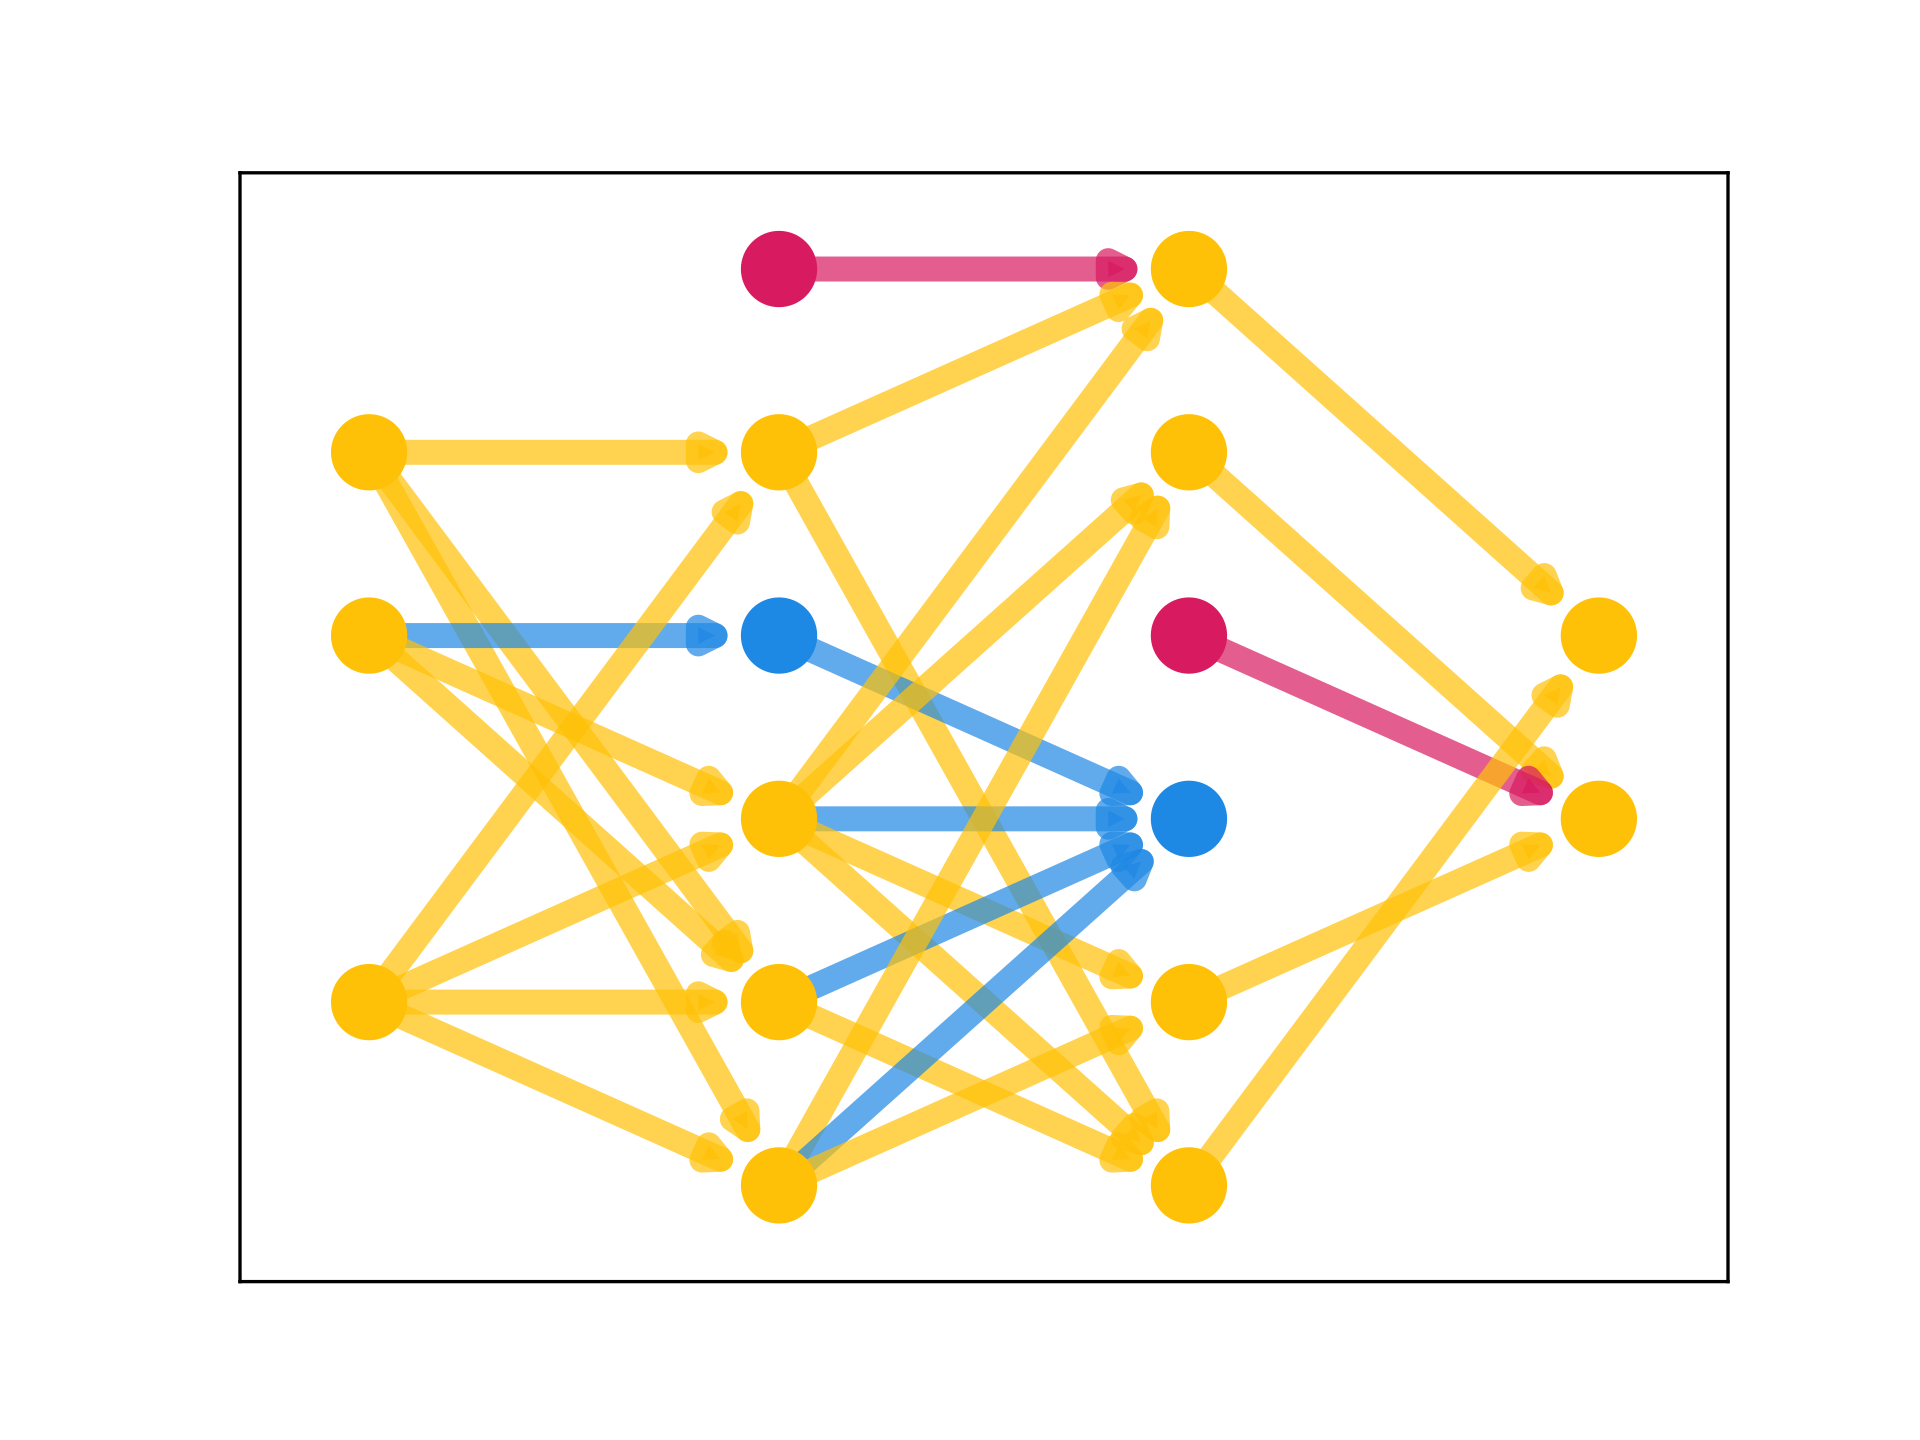
\includegraphics[width=.5\linewidth]{active-example.png}
    \caption[Active, inactive and zombies example]{
    A sample network with active (yellow), inactive (blue) and zombie (magenta) parameters.
    }\label{fig:parameter_categories}
\end{figure}

In figure~\ref{fig:parameter_categories}, the different categories are visualized.
The network input is on the left and the output is on the right.
In magenta, the zombie parameters which are not connected to any input are shown.
In blue, inactive parameters that are not connected to any output are shown.
The rest of the network consists of active parameters in yellow, which are connected to both input and output.
Pruned parameters are not actively visualized, since they are removed from the network.

\subsection{Finding Subnetworks}\label{sec:FindSubnet}
To find independent subnetworks in the network, the previously defined categories are assigned to each parameter after every pruning level.

First, after a network is pruned, each newly pruned weight is tagged as such.
From the directed acyclic graph of the network $\mathcal{G}$ that contains the parameters of all categories a subgraph is created.
Concretely, let $\mathcal{G}$ be defined as the pair $\{V, E\}$, where $V$ is the set of all vertices or nodes and $E$ is the set of all edges.
The set $E_p$ is a subset of $E$, containing all pruned edges of the graph.
The set of unpruned edges is
\[ E_{\neg p} = E - E_p \]
Since biases are not pruned, the set of unpruned nodes is simply $V_{\neg p} = V$
With the vertices $V$ and the unpruned edges $E_{\neg p}$ a subgraph of $\mathcal{G}$ is created, denoted $\mathcal{G}_{\neg p}$.

On this subgraph, $\mathcal{G}_{\neg p}$, inactive nodes and edges are found and assigned their category.
To find inactive parameters, each node except the output nodes is examined.
A node is inactive, if it does not have a valid path to any of the output neurons.
Since the graph is directed, the path is only allowed along the direction of the edge.
Consequently, all incoming edges of an inactive node are also inactive.

The set $E_i$ is a subset of $E_{\neg p}$, and it contains all the inactive edges.
Similarly, the set $V_i$ is a subset of $V$ and contains all the inactive nodes.
All nodes and edges that are neither pruned nor inactive are collected in the sets $V_{\neg i}$ and $E_{\neg i}$ respectively.
They are defined as:
\[ V_{\neg pi} = V_{\neg p} - V_i \]
\[ E_{\neg pi} = E_{\neg p} - E_i \]

The subgraph of $\mathcal{G}_{\neg p}$, which contains only the nodes in $V_{\neg pi}$ and the edges in $E_{\neg pi}$ is denoted $\mathcal{G}_{\neg pi}$.

On the subgraph $\mathcal{G}_{\neg pi}$, which neither contains pruned nor inactive parameters, all zombie parameters are collected.
All nodes, where there is no path from any input to the node, are collected in the set $V_z$.
Further, all edges to or from nodes in the set $V_z$ are collected in $E_z$.
The sets of nodes and edges are defined as:
\[ V_a = V_{\neg piz} = V_{\neg pi} - V_z \]
\[ E_a = E_{\neg piz} = E_{\neg pi} - E_z \]
Because all categories of parameters except for active ones are removed from the sets, they are simply denoted $E_a$ and $V_a$ for short.

With the sets $V_a$ and $E_a$, a new subgraph is created, that represents the active part of the graph $\mathcal{G}$, called $\mathcal{G}_a$.
This active subgraph $\mathcal{G}_a$ is further used to find separated components of the network.

\begin{figure}[ht] % find connected components
\centering
\begin{minipage}{\linewidth}
\begin{lstlisting}[
    language=Python,
    captionpos=b, 
    label={code:split},
    caption={[Finding independent subnetworks]
    Finding independent subnetworks in a neural network with PyTorch~\autocite{networkx} and networkx~\autocite{networkx}; Python pseudo code
    },
]
import torch
import networkx as nx

model: torch.nn.module  #  the neural network

# torch model -> networkx directed acyclic graph
G: nx.DiGraph = transform_to_digraph(model)

# remove pruned, inactive, and zombie parameters
G_not_p = remove_pruned_parameters(G)
G_not_pi = remove_inactive_parameters(G_not_p)
G_a = G_not_piz = remove_zombie_parameters(G_not_pi)

# check for independent subgraphs in the active graph
subnetworks = []
for c in nx.connected_components(G_a.to_undirected()):
    subnetwork = G_a.subgraph(c)
    subnetworks.append(subnetwork)
\end{lstlisting}
\end{minipage}
\end{figure}

The code snippet~\ref{code:split} outlines the process of finding the subnetworks.
A neural network first is converted into a directed acyclic graph.
The network is implemented with PyTorch~\autocite{pytorch}, a commonly used machine learning library and converted into a graph which is further processed with NetworkX~\autocite{networkx}, a well-known library for working with mathematical graphs.
As described previously, the active subgraph \lstinline{G_a} is created.
Connected components of the graph, if there are more than one, are obtained.
A connected component is a subgraph of a graph, where every node is connected via a path to every other node.
Therefore, if the graph is separated, there exist at least two connected components.
The function \lstinline{nx.connected_components}, provided by NetworkX, retrieves all the connected components, which are collected in a list.

\section{Datasets with Independent Tasks}\label{sec:taskmatch}
In this thesis, one area of interest is to see if the network separates given that there exist independent tasks in the dataset.
Critically, it is important to know if the network separates such that it is connected to one task but not the other.
This section explains how the connected components obtained via the methods described in section~\ref{sec:FindSubnet} are then matched to the tasks of the dataset.

\subsection{Definition of Tasks in Datasets}
Consider the dataset $\mathcal{D}$ with its set of input features $\mathcal{D}_X$ and output features or labels $\mathcal{D}_Y$.
Let $T$ be a task, which is defined by the inputs $T_X$ and outputs $T_Y$ that belong to the task, where $T_X$ is a subset of $\mathcal{D}_X$ and $T_Y$ a subset of $\mathcal{D}_Y$.
The tasks $T$ is said to be independent if the set of inputs $T_X$ and outputs $T_Y$ are not shared with any other task.
Independent tasks must not overlap.
Classical machine learning datasets like MNIST~\textcite{mnist} contain one independent task because all input features may be necessary to predict all labels.

However, there can exist datasets with more than one independent task.
Concretely, consider a task $T^{(1)}$ with inputs $T^{(1)}_X$ and outputs $T^{(1)}_Y$ and task $T^{(2)}$ with inputs $T^{(2)}_X$ and outputs $T^{(2)}_Y$.
The sets of inputs $T^{(1)}_X$ and $T^{(2)}_X$ are both subsets of $\mathcal{D}_X$, but are disjoint $T^{(1)}_X \cap T^{(2)}_X = \emptyset$.
The same is true for the input sets.
The set $T^{(1)}_X$ contains information that is relevant to compute the outputs $T^{(1)}_Y$, but no helpful information to compute $T^{(2)}_Y$.
Similarly, the set $T^{(2)}_X$ does not contain information that is useful to compute $T^{(1)}_Y$.
To be able to match networks with tasks, the inputs and outputs of the tasks must be defined alongside the dataset.
Datasets that contain two independent tasks will be created in chapter~\ref{chapter:experiments}.

\subsection{Matching Subnetworks with Tasks}
The subnetworks that are found with the methods described in section~\ref{sec:FindSubnet} now must be matched with the tasks.
For each subnetwork and each task in the dataset, the inputs and outputs of the network are compared to the inputs and labels of the task.

Let $T^{(i)}$ be an independent task that has associated input features in the set $T^{(i)}_X$ and the output features in $T^{(i)}_Y$.
Further, the input and output neurons of a network $j$ are referred to as $N^{(j)}_X$ and $N^{(j)}_Y$ respectively.
For each network and each task, the amount to which the network covers the inputs or outputs of the task can be calculated.
Regarding the inputs, this quantity $c^{(i)}_X$ is referred to as input-coverage. The output-coverage is denoted as $c^{(i)}_Y$.

The number of features that are covered by the network is calculated as the cardinality of the intersection of the network features and the task features $ |N \cap T|$, where  $|A|$ denotes the cardinality of set $A$.
To attain the coverage, the number of features covered by the network is divided by the number of features the task contains.
Then, the coverage is calculated for inputs and outputs as 

\[
c^{(i)}_X = \frac{|N^{(j)}_X  \cap T^{(i)}_X |}{|T^{(i)}_X|} \quad\textit{,where}\quad 0 \leq c^{(i)}_{X} \leq 1\
\]
\[
c^{(i)}_Y = \frac{|N^{(j)}_Y  \cap T^{(i)}_Y |}{|T^{(i)}_Y|} \quad\textit{,where}\quad 0 \leq c^{(i)}_{Y} \leq 1\
\]
Both coverage terms evaluate to $1$ if the network covers all the inputs or outputs of the task.
If the network does not cover any of the inputs or outputs, the input- or output coverage evaluates to $0$ respectively.
The total coverage $c^{(i)}_{XY}$ of the task can be calculated as the product of the input and output coverage.
\[ c^{(i)}_{XY} = c^{(i)}_{X} * c^{(i)}_{Y} \quad\textit{,where}\quad 0 \leq c^{(i)}_{XY} \leq 1\]
The value of the total coverage evaluates to $1$ if both input and outputs are completely covered.
It evaluates to $0$, as soon as either the inputs or outputs are not covered at all.
Depending on the dataset, either of the coverage terms might be used to assess the extent to which the network matches the task.
Consider a scenario where all the inputs and outputs of the task are strictly necessary for the network to perform properly.
Then, the total coverage is a valuable measure.
In a scenario where all outputs are necessary to perform, but not all inputs are important, the output-coverage might be the better measure.

\subsection{Separation, Degradation and Interconnectedness}
Now with the coverages calculated, the network can be categorized.
First, a coverage term that is used for the categorization must be selected.
Consider the network $N$ with $J$ subnetworks $\{N_1, \dots, N_J\}$ and a dataset $\mathcal{D}$ with $K$ tasks $\{T_1, \dots, N_K\}$.
Either the input-, output- or total coverage can be used and will be referred to as $c^{(k)}$ for short, in this section.

The network $N$ is assigned to one of three categories, depending on the coverage of its subnetworks:
\begin{itemize}
    \item \textbf{interconnected}: the network is considered interconnected if the coverage of each task is $1$, but the networks are not separated. Therefore, the number of tasks $K$ is greater than the number of subnetworks $J$.
    An unpruned, fully-connected network is per definition interconnected.
    \[ c^{(k)} = 1; \quad\forall\quad k \in [1, \dots, K]\]
    \[ K > J \]

    \item \textbf{separated}: the network is considered separated if the coverage of each task is $1$, and there is an equal number of subnetworks and tasks.
    \[ c^{(k)} = 1; \quad\forall\quad k \in [1, \dots, K]\]
    \[ K = J \]

    \item \textbf{degraded}: the network is considered degraded if the coverage of at least one task is less than $1$.
    \[ c^{(k)} \leq 1; \quad\textit{for any}\quad k \in [1, \dots, K]\]
\end{itemize}

Concretely, consider a dataset that contains two tasks, $T^{(1)}$ and $T^{(2)}$, with their accociated input sets $T^{(1)}_X$, $T^{(2)}_X$ and output sets $T^{(1)}_Y$, $T^{(2)}_Y$.
Let $J$ denote the number of subnetworks.
The coverages can be collected in a matrix $C$ of size $J \times K$, where $K=2$. 
$c_{j,k}$ represents the value at the $j$-th row and the $k$-th column and $0 \leq c_{j,k} \leq 1$ holds.
The sum of the matrix is upper bound by the number of tasks $K$.
\[ \sum^{i} \sum^{j} c_{j,k} \leq K \]
Given an unpruned network and a dataset with two tasks the matrix would look like the following 
\[ C = \begin{pmatrix} 1 & 1 \end{pmatrix} \]
Each task would be completely covered by the same network.
Since the network per definition covers all tasks before the first pruning level, the matrix will be a unit vector with as many entries as there are tasks.
This network is \textbf{interconnected}.

After several pruning iterations, the network might contain two disconnected subnetworks.
In this case, an additional row is added to the matrix.
For instance, let the subnetworks perfectly match the tasks such that every task is completely covered by one subnetwork.
This network is considered \textbf{separated} and the matrix $C$ might look like the following.
\[ C = \begin{pmatrix} 1 & 0 \\ 0 & 1 \end{pmatrix} \]

After the network is pruned further, all the connections to one of the input nodes might be pruned.
Then, one of the subnetworks would not be completely covered anymore.
This network is considered \textbf{degraded}.
Assuming that half of the features of interest of a given task are not covered anymore, the resulting matrix $C$ would look like the following.
\[ C = \begin{pmatrix} 1 & 0 \\ 0 & 0.5 \end{pmatrix} \]

If the sum of $C$ is equal to the number of tasks and the number of subnetworks is equal to the number of tasks, then the network is (perfectly) separated.
If the sum of $C$ is equal to the number of tasks, but there are fewer subnetworks than tasks, the network still needs to split.
The number of splits that are required can be the difference between the number of tasks and the number of subnetworks.

If the sum of $C$ is less than the number of tasks, the network already has lost at least one input or output.
This scenario is referred to as a degraded network.
Once a network is degraded, a perfect separation cannot be reached anymore.
Generally, throughout this thesis, the training is stopped as soon as the network is degraded to save computational resources.
